\newpage
\section{Revisão da Teoria}

\subsection{Sinalização duobinário}
Nos sistemas de comunicação com modulação por amplitude de pulso (PAM) sinc 
binário, não há interferência inter-simbólica ISI \cite{Lathi}, possuindo 
um desempenho máximo da taxa de sinalização. Porém, um problema apresentado é 
que a resposta em frequência do canal deve ser plana de 0 a $r_b/2$ Hz.

De modo a contornar esse problema, o PAM duobinário insere um ISI conhecido 
para ser interpretado do receptor de uma maneira determinística \cite{Couch}. O 
pulso duibinário satisfaz o critério de Nyquist, pois possui amplitude A em 
$t=0$ e $t=T_b$, com cruzamento em zero em $\pm nT_b (n\neq 0,1)$. Esse pulso 
duobinário ($p_{db}(t)$) pode ser obtido a partir soma de dois pulsos sinc que 
são mostramos no tempo por $T_b$ segundos, de acordo com a equação 
\ref{equ:teo1}.

\begin{equation}
  \label{equ:teo1}
  p_{db}(t) = Asinc \left( \frac{\pi t }{T_b} \right) + Asinc \left( \frac{\pi 
  (t - T_b) }{T_b} \right)
\end{equation} 

O módulo do espectro de tensão $P_{db}(f)$ dos pulsos duobinários é dado pela 
equação \ref{equ:teo2}

\begin{equation}
  \label{equ:teo2}
  P_{db}(f) = 
  \begin{cases}
    2AT_b cos(\pi f T_b), & -\frac{1}{2T_b} \leq f \leq \frac{1}{2T_b} \\
    0, & \mbox{outros casos} 
  \end{cases}
\end{equation}

A densidade espectral de energia bilateral ($E_{db}(f)$) e a densidade 
espectral de potência bilateral ($PSD_{db} (f)$) são dadas pelas equações 
\ref{equ:teo3} e \ref{equ:teo4} \cite{Proakis}, respectivamente.

\begin{equation}
  \label{equ:teo3}
  E_{db}(f) = 
  \begin{cases}
    \frac{2nA^2T_b^2}{R_L}cos^2	(\pi f T_b), & -\frac{1}{2T_b} \leq f \leq 
    \frac{1}{2T_b} \\
    0, & \mbox{outros casos} 
  \end{cases}
\end{equation}

\begin{equation}
  \label{equ:teo4}
  PSD_{db}(f) = 
  \begin{cases}
    \frac{2A^2T_b^2}{R_L}cos^2	(\pi f T_b), & -\frac{1}{2T_b} \leq f \leq 
    \frac{1}{2T_b} \\
    0, & \mbox{outros casos} 
  \end{cases}
\end{equation}

A figura \ref{fig:db} traz uma representação em diagrama de blocos de um 
modulador PAM com sinalização duibinário.

\begin{figure}[H]
    \centering
    \caption{Modulador PAM duobinário.}
    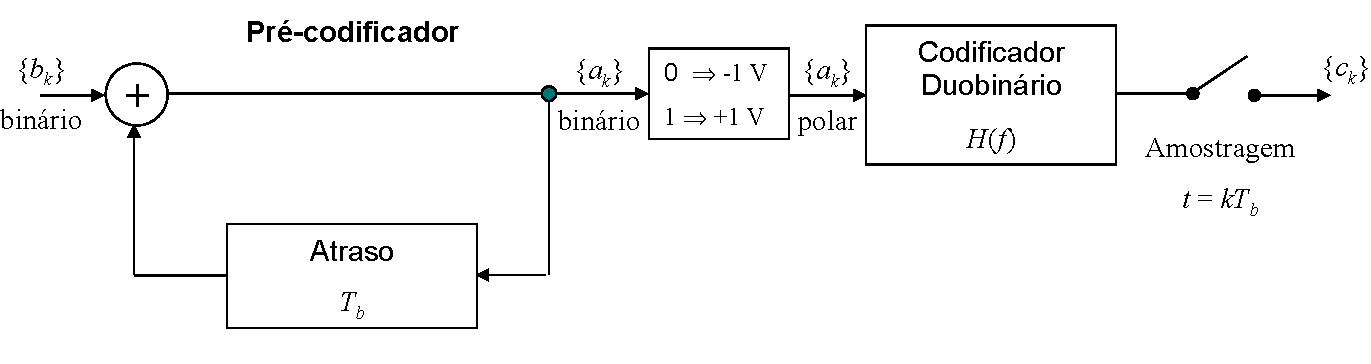
\includegraphics[width=\textwidth]{db}
    \label{fig:db}
\end{figure}

O pulso duobinário tem uma resposta em frequência que não é plana, o que relaxa 
a necessidade de filtros complexos. Assim, pode-se implementar filtros simples 
que se aproximam deste espectro.

\subsection{Sinalização duobinário modificado}

Um outro desafio apresentado tanto pelos pulsos do tipo sinc e duobinários é 
que os mesmos requerem um canal de comunicação que tem uma boa resposta em 
baixa frequência para 0 Hz. Para contornar esse problema é utilizado o pulso 
duiobinário modificado O pulso duobinário modificado. 

O pulso duibinário modificado ($p_{mdb}(t)$) elimina esta preocupação 
\cite{Carlson,Proakis}, podendo ser obtido através da diferença de dois pulsos 
sinc que são mostrados em $2T_b$ segundos, de acordo com a equação 
\ref{equ:teo5}. 

\begin{equation}
\label{equ:teo5}
  p_{mdb}(t) = Asinc \left( \frac{\pi t }{T_b} \right) - Asinc \left( \frac{\pi 
    (t - 2T_b) }{T_b} \right)
\end{equation}

O pulso duibinário modificado satisfaz o critério de Nyquist para não haver 
ISI, pois possui amplitude A em $t=0$ e $t=T_b$, com cruzamento em zero em $\pm 
nT_b (n\neq 0,1)$.

A figura \ref{fig:mdb} traz uma representação em diagrama de blocos do 
modulador PAM com sinalização duobinário modificado.

\begin{figure}[H]
  \centering
  \caption{Modulador PAM duobinário mpodificado.}
  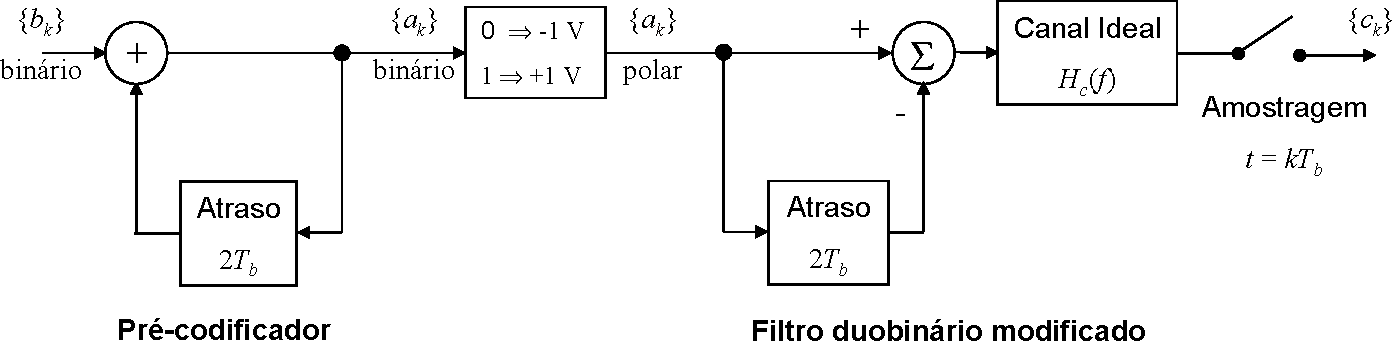
\includegraphics[width=\textwidth]{mdb}
  \label{fig:mdb}
\end{figure}

O módulo do espectro de tensão $P_{mdb}(f)$ dos pulsos duobinários modificados 
é dado pela equação \ref{equ:teo6} \cite{Medeiros}.

\begin{equation}
\label{equ:teo6}
P_{mdb}(f) = 
\begin{cases}
2AT_b sen(\pi f T_b), & -\frac{1}{2T_b} \leq f \leq \frac{1}{2T_b} \\
0, & \mbox{outros casos} 
\end{cases}
\end{equation}

A densidade espectral de potência bilateral ($PSD_{mdb} (f)$) é dada de forma 
similar ao duobinário e está descrita na equação \ref{equ:teo7}.

\begin{equation}
\label{equ:teo7}
PSD_{mdb}(f) = 
\begin{cases}
\frac{2A^2T_b^2}{R_L}cos^2	(\pi f T_b), & -\frac{1}{2T_b} \leq f \leq 
\frac{1}{2T_b} \\
0, & \mbox{outros casos} 
\end{cases}
\end{equation}

